\sse{Continuité de la décomposition lorsque l'on tend vers une application affine}

La décomposition géométrique ne s'applique pas dans le cas des applications affines,  on doit utiliser la méthode multi-étapes. L'expérience suivante montre la continuité de la méthode lorsque l'on considère une suite d'homographies qui converge ponctuellement vers une affinité (cf figure \ref{image_converge_building}). Il n'y a pas de flou ou d'\emph{aliasing} notable juste avant de passer à une affinité, ni de différence visuelle.

\begin{figure}[h!]
		\centering
		\subfigure{
		{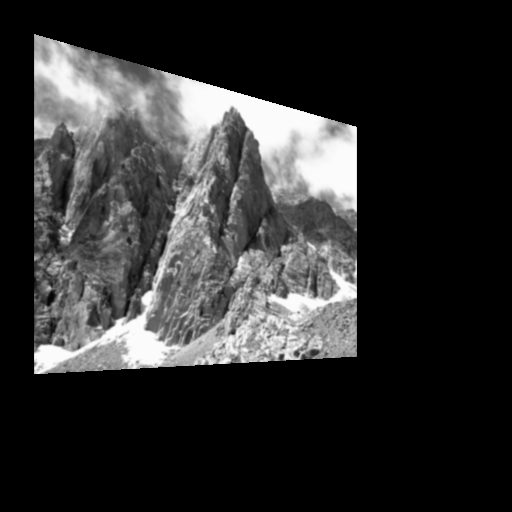
\includegraphics[width=40mm]{test_homo_conv1.png}}
		{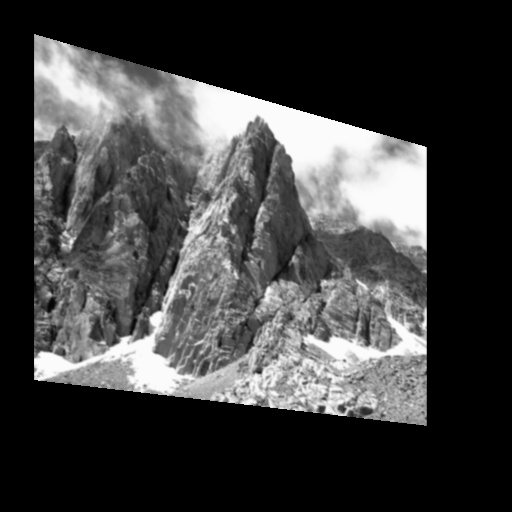
\includegraphics[width=40mm]{test_homo_conv3.png}}
	    {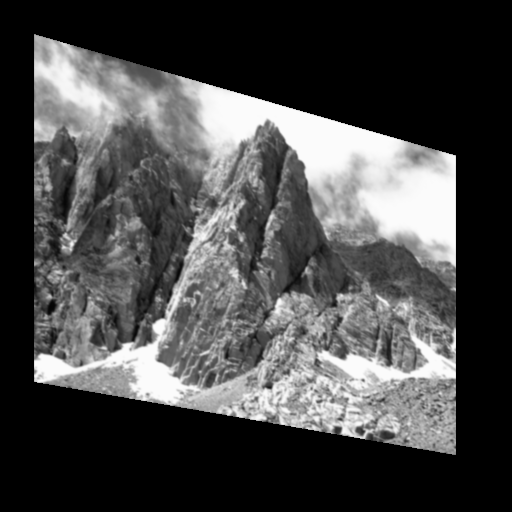
\includegraphics[width=40mm]{test_homo_conv4.png}}}
		\subfigure{
		{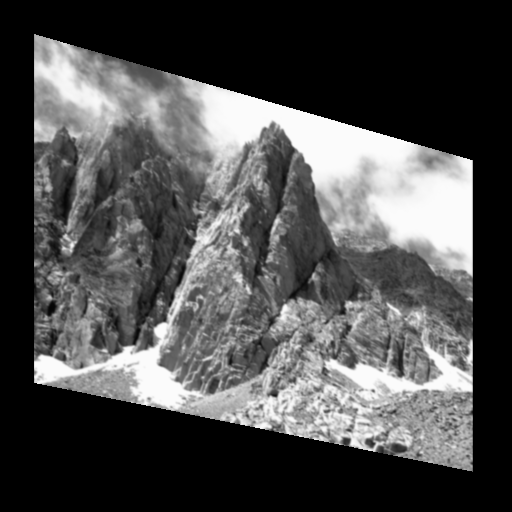
\includegraphics[width=40mm]{test_homo_conv5.png}}
		{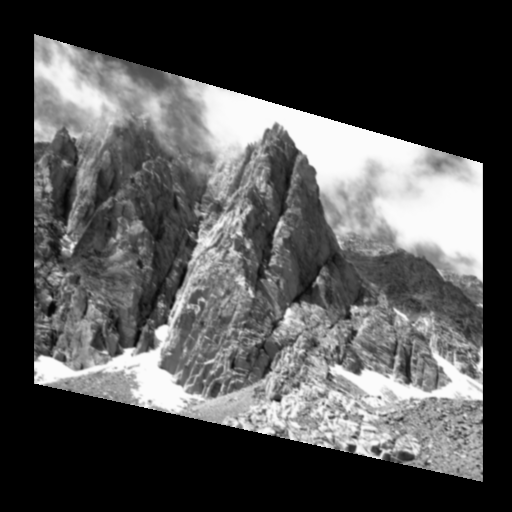
\includegraphics[width=40mm]{test_homo_conv6.png}}
		{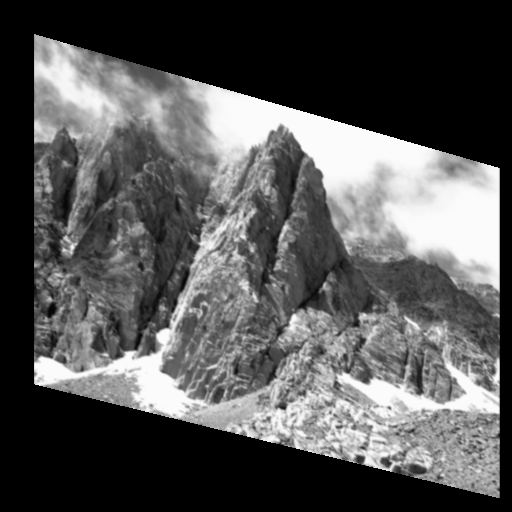
\includegraphics[width=40mm]{test_homo_conv9.png}}}\\
		\caption{Convergence vers une application affine ; la dernière image est la limite}
\label{image_converge_building}
\end{figure}
